%
% CURVAS ELÍPTICAS
%
\section{Curvas Elípticas}

\subsection{Definição}
Curvas elípticas não são elipses. Elas têm esse porque são descritas por equações cúbicas, semelhantes às usadas para calcular a circunferência de uma elipse. Em geral, as equações cúbicas para curvas elípticas têm a forma
\begin{equation}
y^2 + axy + by = x^3 + cx^2 + dx + e \label{eq:5}
\end{equation}
onde \(a, b, c, d\) e \(e\) são números reais e \(x\) e \(y\) assumem valores nos números reais. Equações deste tipo são chamadas de \textit{equações de Weiestrass}. Para a nossa finalidade, é suficiente limitarmos na forma normal da equação de Weiestrass
\begin{equation}
y^2 = x^3 + ax + b \label{eq:6}
\end{equation}

Essas equações são consideradas cúbicas, ou de grau 3, pois o expoente mais alto que elas contém é um 3. Também incluído na definição de uma curva elíptica está um único elemento indicado por \(O\) e chamado de \textit{ponto no infinito} ou \textit{ponto zero}.

A Figura \ref{fig:curvas} apresenta alguns exemplos de curvas elípticas usando a forma normal da equação de Weierestrass.

\begin{figure}[h]
\centering
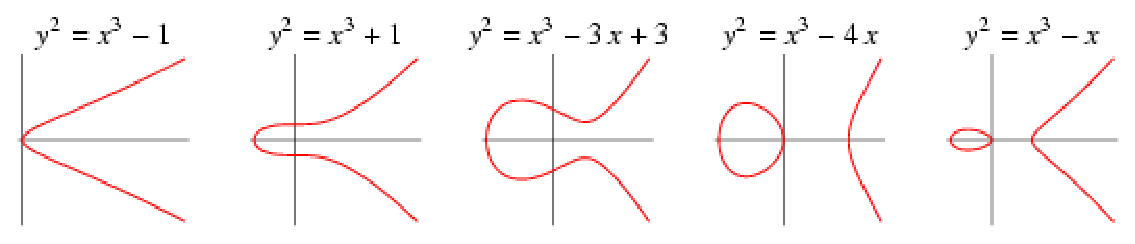
\includegraphics[scale=0.5, bb=0 0 529 101]{figuras/curvas.eps}
\caption{Exemplos de curvas elípticas}
\label{fig:curvas}
\end{figure}

Podemos mostrar que um grupo pode ser definido com base no conjunto E(\(a, b\)) para valores específicos de \(a\) e \(b\) na Equação \ref{eq:6}, desde que a condição a seguir seja atendida:
\begin{equation}
4a^3 + 27b^2 \neq 0 \label{eq:7}
\end{equation}

\subsection{Propriedades}
Uma importante característica da curvas elípticas é que existe uma forma natural de ``somar'' dois pontos produzindo um terceiro ponto. Para tanto, deve-se satisfazer a Equação \ref{eq:7}. No entanto, esta ``soma'' se refere à operação que combina dois pontos de maneira análoga da soma algébrica em alguns aspectos (é comutativa, associativa e existe um elemento identidade), mas bem diferente em outras formas.

Em termos geométricos, as regras para a adição podem ser indicadas da seguinte maneira: se três pontos em uma curva elíptica se encontram em uma linha reta, sua soma é \(O\). Por essa definição, podemos definir as regras da adição sobre uma curva elíptica:

\begin{figure}[h]
\centering
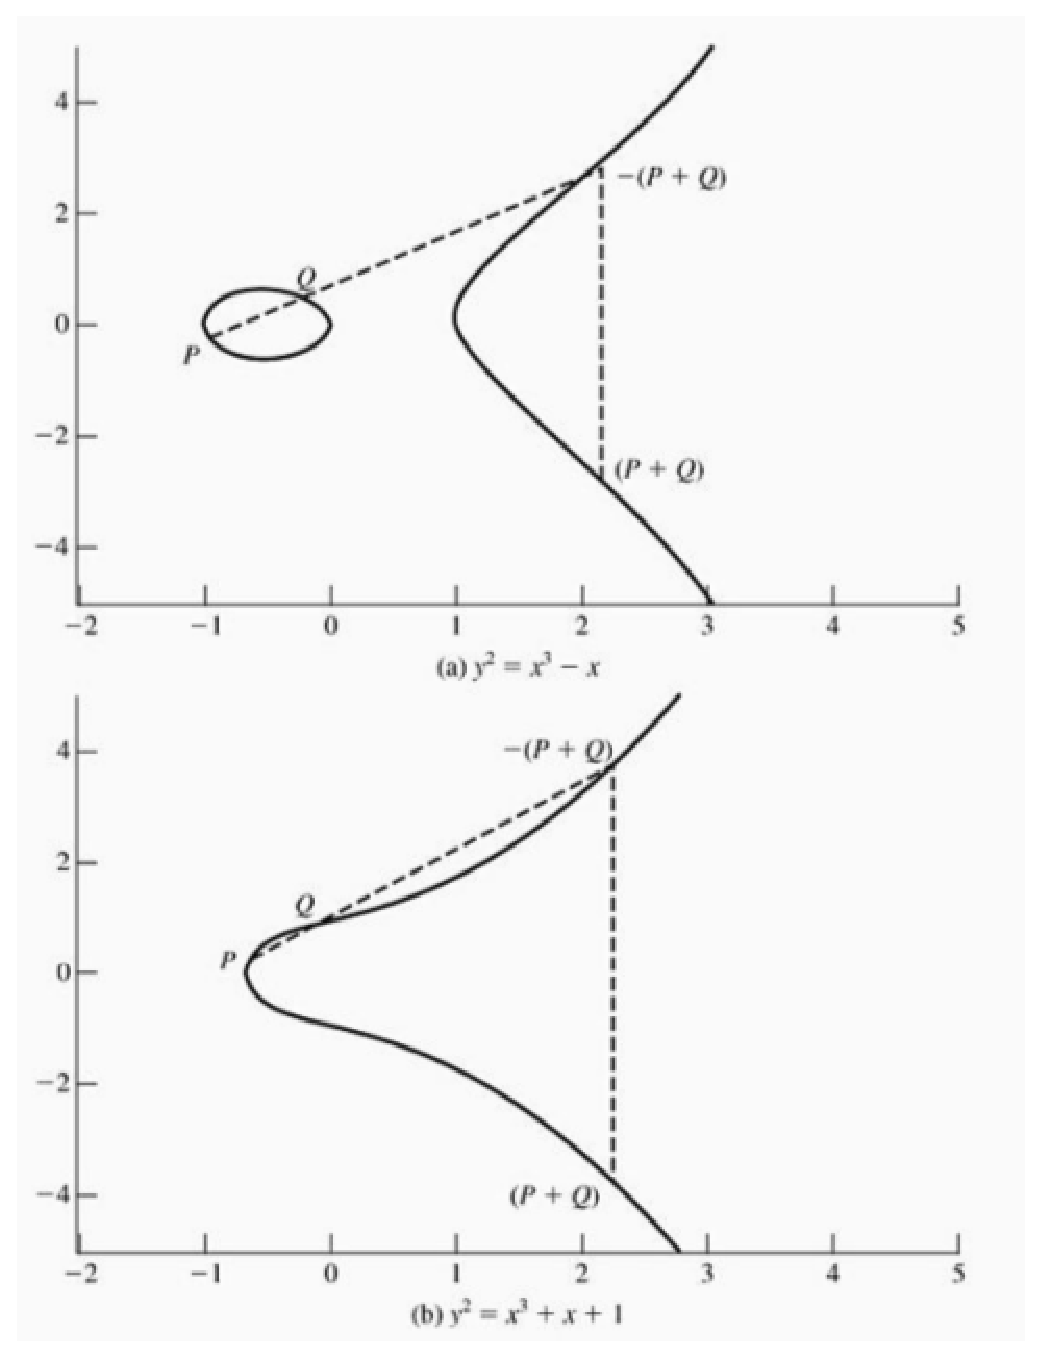
\includegraphics[scale=0.5, bb=0 0 484 636]{figuras/pontos_curva.eps}
\caption{Exemplos de soma de pontos em curvas elípticas}
\label{fig:pontos}
\end{figure}

\begin{enumerate}
  \item $O$ funciona como a identidade aditiva. Assim, $O = -O$; para qualquer ponto $P$ na curva elíptica, $P + O = P$. A seguir, consideramos $P \neq O$ e $Q \neq O$.
  \item O negativo de um ponto \(P\) é o ponto com a mesma coordenada \(x\), sem o negativo da coordenada \(y\); ou seja, se $P = (x, y)$, então $-P = (x, -y)$. Observe que esses dois pontos podem ser juntados por uma linha vertical. Observe que $P + (-P) = P - P = O$.
  \item Para somar dois pontos \(P\) e \(Q\) com coordenadas \(x\) diferentes, desenhe uma linha reta entre eles e encontre o terceiro ponto de interseção \(R\). Pode-se ver facilmente que existe um único ponto \(R\) que é o ponto de interseção (a menos que a linha seja tangente à curva em \(P\) ou \(Q\), quanto consideramos $R=P$ ou $R=Q$, respectivamente). Para formar uma estrutura de grupo, precisamos definir a adição sobre três pontos da seguinte forma: $P+Q=-R$. Ou seja, definimos $P+Q$ como sendo a imagem-espelho (com relação ao eixo \(x\)) do terceiro ponto da interseção. A figura \ref{fig:pontos}
  \item A interpretação geométrica do item anterior também se aplica a dois pontos, \(P\) e \(-P\), com a mesma coordenada \(x\). Os pontos são reunidos por uma linha vertical, que também pode ser vista como a interseção da curva no ponto infinito. Portanto, temos $P+(-P)=O$, coerente com o item (2).
  \item Para dobrar um ponto \(Q\), desenhe uma linha tangente e encontre o outro ponto da interseção \(S\). Então, $Q+Q=2Q=-S$.
\end{enumerate}

Com a lista de regras apresentada, pode-se se mostrar que o conjunto E(\(a, b\)) é um grupo abeliano. \cite{Stallings:2011}

\subsection{Curvas elípticas sobre corpo finito}
A criptografia de curva elíptica utiliza curvas elípticas em que as variáveis e coeficientes são todos restritos a elementos de um corpo finito, ou seja, assumem valores no conjunto de inteiros de 0 até $p - 1$ em que os cálculos são realizados módulo \(p\). Desta forma, é dito que a curva está sobre $\mathbb{F}_p$. \cite{Stallings:2011}

\begin{equation}
y^2 \mod p = (x^3 + ax + b) \mod p
\end{equation}

Pode-se mostrar que um grupo abeliano finito é definido com base no conjunto $E_p(a, b)$, desde que $(x^3 + ax + b) \mod p$ não tenha fatores repetidos. Isso é equivalente à condição

\begin{equation}
(4a^3 + 27b^2) \mod p \neq 0 \label{eq:13}
\end{equation}

A Equação \ref{eq:13} tem a mesma forma da Equação \ref{eq:7}. As regras para adição sobre $E_p(a, b)$ correspondem à técnica algébrica descrita para as curvas elípticas definidas sobre números reais. Para todos os pontos $P, Q \in E_p(a, b)$.

\begin{figure}[h]
\centering
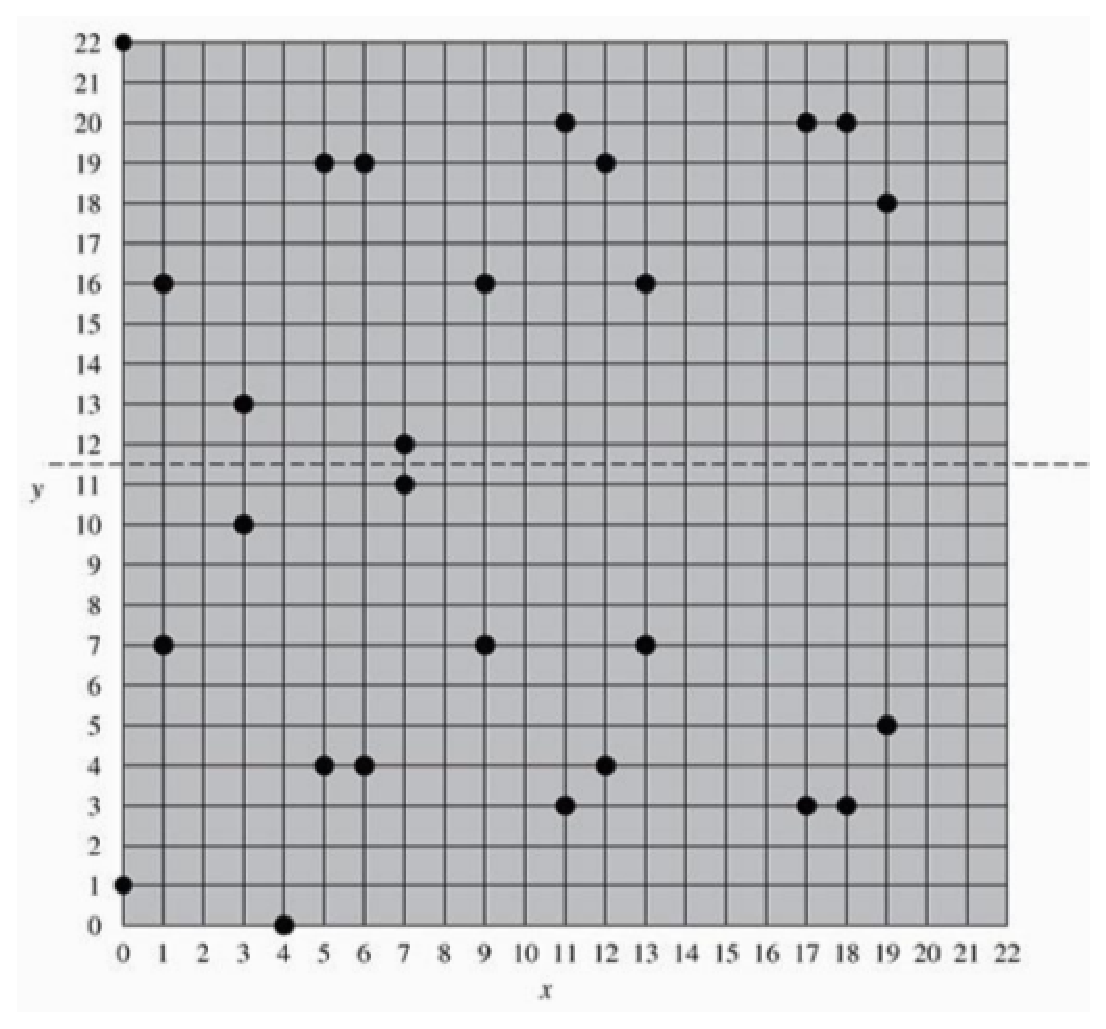
\includegraphics[scale=0.6, bb=0 0 515 478]{figuras/curva_sobre_corpo_finito.eps}
\caption{Curva elíptica $E_{23}(1, 1)$}
\label{fig:curvas}
\end{figure}

\begin{enumerate}
  \item $P + O = P$.
  \item Se $P = (x_P, y_P)$, então $P + (x_P, -y_P) = O$. O ponto $(x_P, -y_P)$ é o negativo de \(P\), indicado como \(-P\).
  \item Se $P = (x_P, y_P)$ e $Q = (x_Q, y_Q)$ com $P \neq -Q$, então $R = P + Q = (x_R, y_R)$ é determinado pelas seguintes regras:
    \begin{eqnarray*}
    x_R &=& (\lambda^2 - x_P - x_Q) \mod p \\
    y_R &=& (\lambda(x_P - x_R) - y_P) \mod p
    \end{eqnarray*}
  onde
    \begin{eqnarray*}
    \lambda =
    \begin{cases}
    \left(\dfrac{y_Q - y_P}{x_Q - x_P}\right) \mod p \textrm{, se} \ P \neq Q \\ \\
    \left(\dfrac{3x_P^2 + a}{2y_P}\right) \mod p \textrm{, se} \ P = Q
    \end{cases}
    \end{eqnarray*}
  \item A multiplicação é definida como adição repetida; por exemplo, $4P = P + P + P + P$.
\end{enumerate}

%
% ECDPL
%
\subsection{O problema do logaritmo discreto sobre curvas elípticas} \label{ecdpl}
Seja \(E\) uma curva elíptica sobre o corpo finito $\mathbb{F}_p$ e seja \(P\) e \(Q\) pontos em $E_p(a, b)$. O problema do logaritmo discreto sobre curvas elípticas ECDLP (\textit{Elliptic Curve Discrete Logarithm Problem}) é o problema de encontrar um inteiro \(n\) tal que $Q = nP$. Pela analogia com o problema do logaritmo para $\mathbb{F}_p^*$, denotamos esse inteiro \(n\) por

\begin{eqnarray}
nP &=& Q \label{eq:ecdpl1} \\
n &=& \log_P(Q) \label{eq:ecdpl2}
\end{eqnarray}

e chamamos \(n\) como logaritmo discreto elíptico de \(Q\) em relação a \(P\). \cite{Hoffstein:2008}

\subsection{Algoritmos conhecidos para resolver ECDPL}
Ataques mais conhecidos sobre ECC têm complexidade exponencial. Essa afirmação é válida para curvas genéricas e exclui ataques em subclasses especiais, como curvas supersingular e anômalo. A solução para a Equação \ref{eq:ecdpl2} pode ser calculada usando as seguintes técnicas: \cite{Pelzl:2006}

\begin{itemize}
\item Força-bruta: Este método adiciona sequencialmente o ponto $P \in E(\mathbb{F}_p)$ a ele mesmo. A cadeia de adição $P, 2P, 3P, 4P, ...$ acabará por chegar em \(Q\) descobrindo assim o valor de \(n\), de acordo com a Equação \ref{eq:ecdpl1}. No pior caso, este cálculo pode levar a $n - 1$ passos onde \(n\) é da ordem de \(P\). Desta forma, o ataque pode se tornar inviável para prática quando \(n\) é muito grande.
\item \textit{Baby Step Giant Step} (BSGS): O algoritmo BSGS é uma melhoria à busca por força-bruta. Para \(n\) na ordem de \(P\), memória temporária por cerca de $\sqrt{n}$ e aproximadamente um adicional de $\sqrt{n}$ passos são necessários. No entanto, devido à sua complexidade de memória alta, BSGS acaba não sendo muito interessante.
\item Pollard's Rho: O ataque Pollard Rho foi proposto por J. Pollard em 1978 e é um algoritmo baseado em colisão com base em um percurso aleatório num grupo cíclico, assim, pode ser aplicado ao grupo de pontos gerados por \(P\) numa curva elíptica. O percurso aleatório calcula uma trilha de pontos numa curva elíptica e eventualmente termina em um ciclo, revelando a solução para ECDLP. Embora tendo um tempo de complexidade similar de $\sqrt{\pi n/2}$ comparado ao BSGS, Pollard's Rho é superior devido aos seus desprezíveis requisitos de memória. Em combinação com a paralelização adequada, o método Pollard's Rho é o mais rápido ataque conhecido contra ECC. Neste trabalho serão apresentados os métodos Pollard's Rho original, Pollard's Rho com único processador (SPPR), e sua variante paralelizada Pollard's Rho com multi-processadores (MPPR).
\end{itemize}

%
% CRIPTOGRAFIA DE CURVAS ELÍPTICAS
%
\subsection{Criptografia de curvas elípticas}
Primeiro, selecione um inteiro grande \(p\) que seja primo e parâmetros da curva elíptica \(a\) e \(b\) de acordo com a equação \ref{eq:5} ou \ref{eq:6}. Isso define o grupo elíptico de pontos $E_q(a, b)$. Em seguida escolha um ponto base $G = (x_1, y_1)$ em $E_q(a, b)$, cuja a ordem seja um valor muito grande \(n\). $E_q(a, b)$ e \(G\) são os parâmetros do criptossistema, conhecidos por todos os participantes.

Um acordo de chaves entre os usuários A e B pode ser realizado da seguinte maneira:
\begin{enumerate}
\item \textbf{A} seleciona um inteiro \(n_A\) menor que \(n\). Essa é chave privada de \textbf{A}, então \textbf{A} gera sua chave pública $P_A = n_A \times G$
\item Do mesmo modo, \textbf{B} seleciona um inteiro \(n_B\) menor que \(n\), sendo essa a chave privada de \textbf{B}. E então \textbf{B} calcula e divulga sua chave pública $P_B = n_B \times G$.
\item \textbf{A} gera a chave secreta $k = n_A \times P_B$. \textbf{B} gera a chave secreta $k = n_B \times P_A$
\end{enumerate}

Os dois cálculos na etapa 3 produzem o mesmo resultado, porque
\begin{equation*}
n_A \times P_B = n_A \times (n_B \times G) = n_B \times (n_A \times G) = n_B \times P_A
\end{equation*}

Para quebrar esse esquema, um atacante teria de ser capaz de calcular \(k\) a partir de \(kG\), o que é considerado difícil. Este problema que é conhecido como problema do \textit{\textbf{logaritmo discreto sobre curvas elípticas}}, como já explicado em \ref{ecdpl}.
